\documentclass{article}

\usepackage[margin=1in]{geometry}
\usepackage{graphicx}

\begin{document}
\begin{titlepage}
	\clearpage\thispagestyle{empty}
	\centering
	\vspace{1cm}

	\rule{\linewidth}{1mm} \\[0.5cm]
	{ \Large \bfseries ISyE 6740 - Fall 2023\\[0.2cm]
		Final Report}\\[0.5cm]
	\rule{\linewidth}{1mm} \\[1cm]

		\begin{tabular}{l p{5cm}}
		\textbf{Team Member Names:} David Nguyen - 3593, Jorge Banegas - 7136, Thomas Algenio - 4379&  \\[10pt]
  		\textbf{Group Number:} 95 &  \\[10pt]
		\textbf{Project Title:} Decomposing and Classifying Real and Photoshopped Face Images &  \\[10pt]
		\end{tabular}

        \begin{itemize}
            \item[] \textbf{Problem Statement}

            With the growing popularity of AI, countless positive contributions have been made to solve the world's toughest challenges. Along with these vast contributions to science and technology, there are also growing pain points when individual users leverage AI. In this research paper, we'll discuss the growing concerns within the computer vision category of AI. Although there are benefits of wanting to use AI to manipulate images (sharpening historical photos, facial recognition for identity verification, etc.), there are also reasons to use image manipulation techniques maliciously. A modern-day problem that has recently started becoming increasingly popular is the ability to create fake images of individuals that seem virtually realistic. This could lead to many adverse and undesirable effects for an individual.

            Facial recognition has emerged as a pivotal technology in various sectors, from security and surveillance to personalized user experiences in digital platforms. However, with the proliferation of sophisticated image manipulation tools and generative models, the challenge of distinguishing genuine faces from artificially generated or manipulated ones has become paramount. Ensuring the accuracy and reliability of facial recognition systems in the face of these challenges is crucial. This paper aims to understand better the complexities of classifying these image types and evaluate techniques that will lead to reasonable classification rates.

            \item[] \textbf{Data Source}

\begin{figure}[H]
\caption{Easy Level Fake Images}
\centering
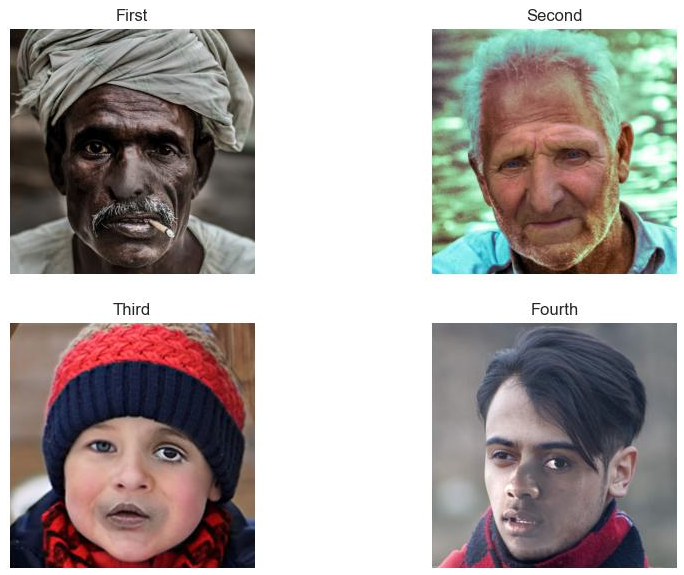
\includegraphics[width = 0.325\textwidth]{4_img_easy.png}
\caption{Medium Level Fake Images}
\centering
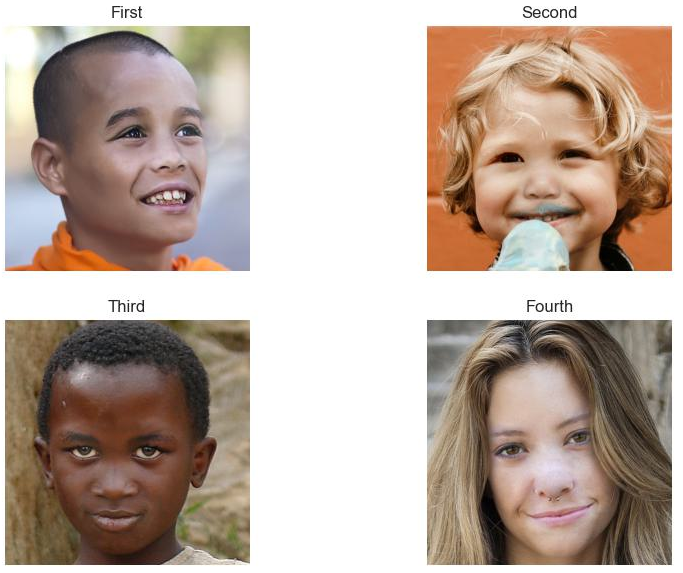
\includegraphics[width = 0.325\textwidth]{4_img_med.png}
\caption{Hard Level Fake Images}
\centering
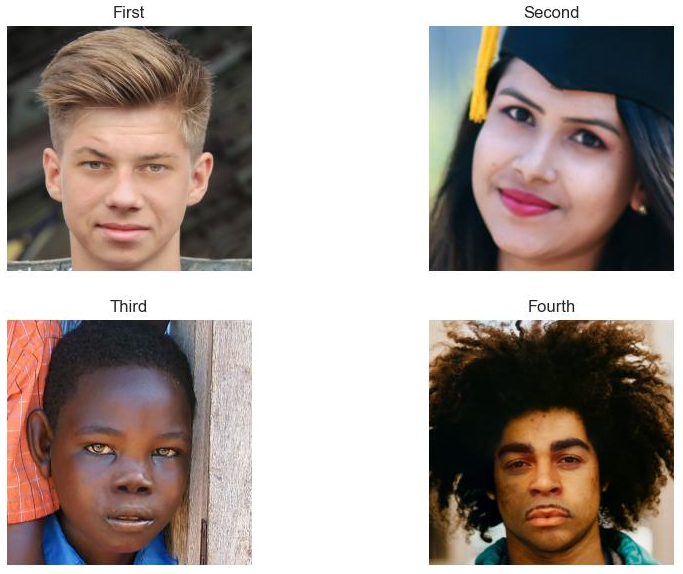
\includegraphics[width = 0.325\textwidth]{4_img_hard.png}
\caption{Real Images}
\centering
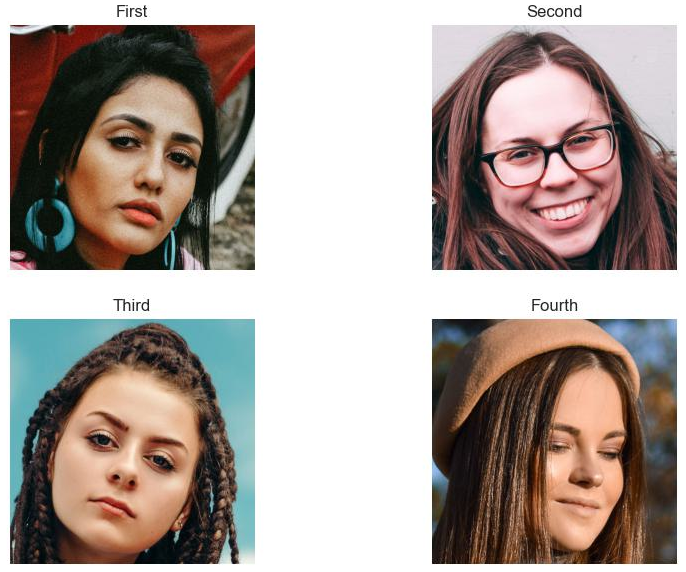
\includegraphics[width = 0.325\textwidth]{4_img_real.png}
\end{figure}

            Seonghyeon Nam, Seoung Wug Oh, Jae Yeon Kang, Chang Ha Shin, Younghyun Jo, Young Hwi Kim, Kyungmin Kim, Minho Shim, Sungho Lee, Yunji Kim, Suho Han, Gunhee Nam, Dasol Lee, Subin Jeon, In Cho, Woongoh Cho, Sejong Yang, Dongyoung Kim, Hyolim Kang, Sukjun Hwang, and Seon Joo Kim. (2019, January). Real and Fake Face Detection, Version 1. Retrieved [2023, September 19] from https://www.kaggle.com/datasets/ciplab/real-and-fake-face-detection.

\begin{center}
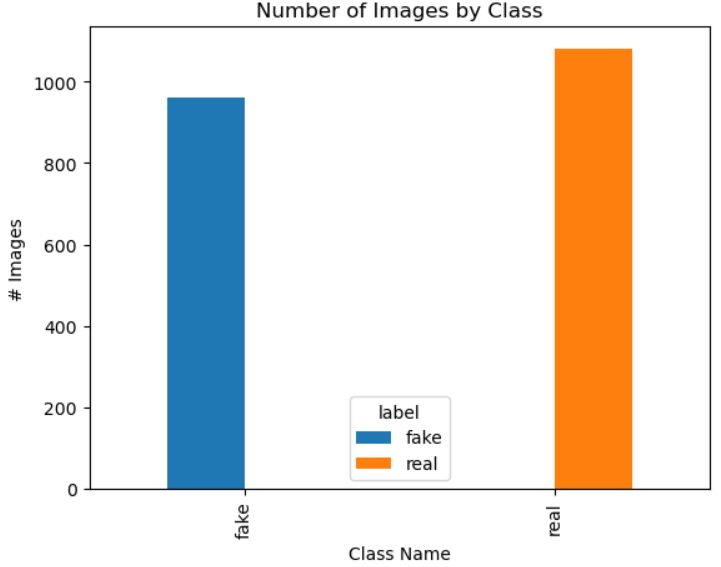
\includegraphics[width = 0.375\textwidth]{balance_histogram.png}
\end{center}

\newpage

    \textbf{Data Preprocessing}




Data preprocessing from original RGB images to black and white 1D arrays involves several key steps to convert the input data into a format suitable for machine learning models. Here's a summary of the process:

\textbf{Loading the Images:}

We begin by loading the original RGB images into our environment using PIL and then convert to Grayscale. Grayscale images are single channels that represent the intensity of light versus the RGB images, which have 3 channels to represent the intesnity of each RGB color.


\textbf{Normalization:}

We Normalize the pixel values of the grayscale images. This step involves scaling the pixel values to a range between 0 and 1, making it easier for the model to learn.

\textbf{Resizing:}

Our machine learning models expect a consistent input size, so we have to revise out datasize to have a ($600$ x $600$) dimensional matrix.
Flattening:

We can flatten the 2D grayscale images into 1D arrays. This involves reshaping the image matrix into a vector. The initial size is (height x width), the flattened array will have size (height * width,).


\textbf{Feature Scaling:}

We scale the pixel values of the flattened arrays. We do this in order to normalize the data when working with image data.

\textbf{Data Splitting:}

We then split our data set into training and testing data splits. All of our accuracy scores are evaluated and calculated on the "testing" (unseen) data, helping to identify model performance. We will bedoing an 80/20 split on our dataset, which equates to around a training set of

\textbf{Data Summary:}

Our final data set matrix size came out to be (2,401 x 360,000). 2,401 represents the total number of images we had, and 360,000 represents that total pixel size of each image as they were flattened.

\newpage

% 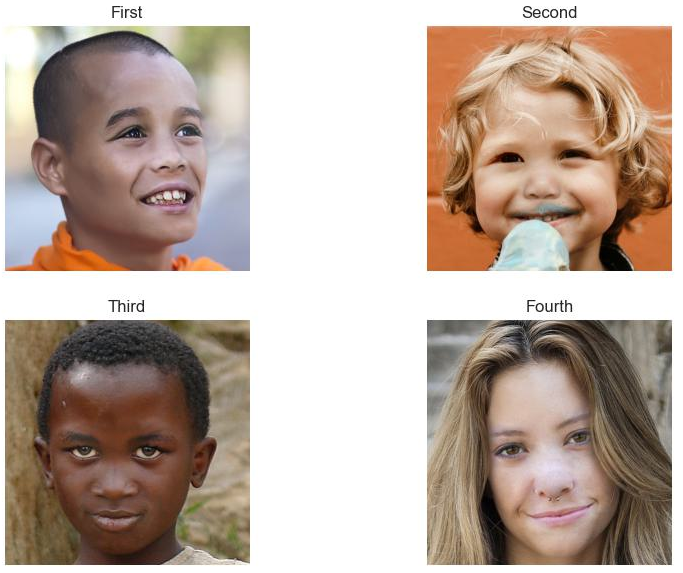
\includegraphics[width = 0.4\textwidth]{4_img_med.png}
% \end{center}

\newpage

\textbf{Methodology: PCA and ISOMAP Dimensionality Reduction}

We will test different dimensionality reduction algorithms and plot the images on a 2-D subspace. This will allow us to visualize similar pictures on a two-dimensional plot. We expect a separated plot between real and fake image classes from our project proposal. PCA focuses on capturing variance and providing a linear transformation of the data, whereas ISOMAP emphasizes preserving non-linear relationships and the geometry of the data. The choice between PCA and ISOMAP depends on the data's underlying structure and the analysis's goals.

\begin{center}
    \includegraphics[width=0.645\linewidth]{pca_projection.png}
\end{center}

\begin{center}
    \includegraphics[width=0.625\linewidth]{variance_exp.png}
\end{center}

\begin{center}
    \includegraphics[width=0.645\linewidth]{iso_projection.png}
\end{center}

For dimensionality reduction, our primary focus was visualizing a higher dimensional data set on a 2D space. This allows for greater interpretability of our data set and the associated feature space due to the more intuitive visualizations of the data points and their positions. Although dimensionality reduction has benefits, depending on the project's end state, it may only sometimes be optimal. For our classification problem, we would like to maximize our classification scores to assign a solution to a modern-day problem.

Some of the drawbacks of dimensionality reduction include the significant loss in variability. Our variation bar plot shows that reducing the variable space to 10 dimensions only explains about $63\%$ of the variability within the data set. When we calculate the variability explained for our 2D space, we see a percentage around $38\%$. The significant loss of information will reflect on the classification/purity scores from our lower dimensional data sets.

To have a balance between model simplicity and loss of variability, we went ahead. We tested the number of dimensions that could explain at least $80\%$ of the variance within our data set, which is around \textbf{50 dimensions}, compared to the original 360,000 feature array.

\begin{center}
    \includegraphics[width=0.55\linewidth]{variance_bat.png}
\end{center}
\newpage

    \textbf{Method 1: Unsupervised Clustering}

    Initial ad-hoc analysis for unsupervised clustering, we are looking to use K-Means to search for photos that share similar features. To assess model accuracy, we can calculate the purity of each cluster by obtaining the number of images of real or fake photos out of all data points in each cluster set. We will treat this method as an unsupervised learning method to understand how the different image types are clustered. Ideally, fake images will be clustered similarly to each other, as well as authentic images.

\textbf{Running classification models with reduced 2-dimensions PCA}

For our \textbf{KMeans} Clustering Model, we obtain the following:

\begin{verbatim}
True Positives: 134
True Negatives: 90
False Positives: 84
False Negatives: 101
              precision    recall  f1-score   support

           0       0.47      0.52      0.49       174
           1       0.61      0.57      0.59       235

    accuracy                           0.55       409
   macro avg       0.54      0.54      0.54       409
weighted avg       0.55      0.55      0.55       409

Specificity 0.52
Accuracy: 54.768%
AUC:  0.5437270726338959
\end{verbatim}



\textbf{Running classification models with reduced 50-dimensions PCA}

For our \textbf{KMeans} Clustering Model, we obtain the following:

\begin{verbatim}
True Positives: 160
True Negatives: 122
False Positives: 58
False Negatives: 69
              precision    recall  f1-score   support

           0       0.58      0.61      0.60       180
           1       0.64      0.67      0.68       229

    accuracy                           0.64       409
   macro avg       0.64      0.64      0.64       409
weighted avg       0.65      0.64      0.64       409

Specificity 0.61
Accuracy: 57.279%
AUC:  0.5693983503153809
\end{verbatim}

\textbf{Running classification models with reduced 2-dimensions ISOMAP}

For our \textbf{KMeans} Clustering Model, we obtain the following:

\begin{verbatim}
True Positives: 122
True Negatives: 100
False Positives: 96
False Negatives: 91
              precision    recall  f1-score   support

           0       0.52      0.51      0.52       196
           1       0.56      0.57      0.57       213

    accuracy                           0.54       409
   macro avg       0.54      0.54      0.54       409
weighted avg       0.54      0.54      0.54       409

Specificity 0.51
Accuracy: 54.279%
AUC:  0.5414870173421481
\end{verbatim}

\textbf{Running classification models with reduced 50-dimensions ISOMAP}

For our \textbf{KMeans} Clustering Model, we obtain the following:

\begin{verbatim}
True Positives: 152
True Negatives: 129
False Positives: 66
False Negatives: 62
              precision    recall  f1-score   support

           0       0.52      0.51      0.54       195
           1       0.58      0.57      0.60       214

    accuracy                           0.57       409
   macro avg       0.54      0.54      0.57       409
weighted avg       0.55      0.54      0.58       409

Specificity 0.61
Accuracy: 58.034%
AUC:  0.5788928828181164
\end{verbatim}

In both of our dimensionality reduction algorithms, when we reduce our dimensions to 2 feature vectors, there isn't a discernible pattern within each real and fake class. Based on our analytical results, we noticed that when we projected our image matrix on a two-dimensional vector space, our classification models performed as well as around ($54\%$), which is slightly better than guessing real/fake images. However, when we decomposed the feature space into 50 dimensions, we saw significantly greater performance on our classification scores $(64.3\%)$.

\newpage


    \textbf{Method 2: Labeled Classification}

    Instead of a clustering algorithm, we decided to leverage classification models because we have a labeled set of real and fake images. Classification models that we will be using are: logistic regression, random forest classification, and XGBoost model. We can calculate the most notable binary classification metrics to assess model accuracy. We will treat this method as supervised learning to understand if the images can be mathematically separated into different groupings. Ideally, there will be a clear delineation between real and fake face image groups.


\textbf{Running classification models with reduced 2-dimensions PCA/ISOMAP}

For our \textbf{Logistic Regression} Classification Model, we obtain the following:

\begin{verbatim}
True Positives: 201
True Negatives: 25
False Positives: 166
False Negatives: 17
              precision    recall  f1-score   support

           0       0.60      0.13      0.21       191
           1       0.55      0.92      0.69       218

    accuracy                           0.55       409
   macro avg       0.57      0.53      0.45       409
weighted avg       0.57      0.55      0.47       409

Specificity 0.13
Accuracy: 55.257%
AUC:  0.5264542004899371
\end{verbatim}

For our \textbf{Random Forest} Classification Model, we obtain the following:

\begin{verbatim}
True Positives: 109
True Negatives: 93
False Positives: 98
False Negatives: 109
              precision    recall  f1-score   support

           0       0.46      0.49      0.47       191
           1       0.53      0.50      0.51       218

    accuracy                           0.49       409
   macro avg       0.49      0.49      0.49       409
weighted avg       0.50      0.49      0.49       409

Specificity 0.49
Accuracy: 49.389%
AUC:  0.49345549738219896
\end{verbatim}

For our \textbf{XGBoost} Classification Model, we obtain the following:

\begin{verbatim}
True Positives: 116
True Negatives: 95
False Positives: 96
False Negatives: 102
              precision    recall  f1-score   support

           0       0.48      0.50      0.49       191
           1       0.55      0.53      0.54       218

    accuracy                           0.52       409
   macro avg       0.51      0.51      0.51       409
weighted avg       0.52      0.52      0.52       409

Specificity 0.5
Accuracy: 51.589%
AUC:  0.5147461453479995
\end{verbatim}

\textbf{Running classification models with reduced 50-dimensions PCA/ISOMAP}

For our \textbf{Logistic Regression} Classification Model, we obtain the following:

\begin{verbatim}
True Positives: 156
True Negatives: 107
False Positives: 84
False Negatives: 62
              precision    recall  f1-score   support

           0       0.63      0.56      0.59       191
           1       0.65      0.72      0.68       218

    accuracy                           0.64       409
   macro avg       0.64      0.64      0.64       409
weighted avg       0.64      0.64      0.64       409

Specificity 0.56
Accuracy: 64.303%
AUC:  0.6379028771794996
\end{verbatim}

For our \textbf{Random Forest} Classification Model, we obtain the following:

\begin{verbatim}
True Positives: 151
True Negatives: 87
False Positives: 104
False Negatives: 67
              precision    recall  f1-score   support

           0       0.56      0.46      0.50       191
           1       0.59      0.69      0.64       218

    accuracy                           0.58       409
   macro avg       0.58      0.57      0.57       409
weighted avg       0.58      0.58      0.58       409

Specificity 0.46
Accuracy: 58.191%
AUC:  0.5740789663288342
\end{verbatim}

For our \textbf{XGBoost} Classification Model, we obtain the following:

\begin{verbatim}
True Positives: 147
True Negatives: 97
False Positives: 94
False Negatives: 71
              precision    recall  f1-score   support

           0       0.58      0.51      0.54       191
           1       0.61      0.67      0.64       218

    accuracy                           0.60       409
   macro avg       0.59      0.59      0.59       409
weighted avg       0.59      0.60      0.59       409

Specificity 0.51
Accuracy: 59.658%
AUC:  0.591082664873433
\end{verbatim}


In both of our dimensionality reduction algorithms, when we reduce our dimensions to 2 feature vectors from the flattened (600 x 600) image, there isn't a discernible pattern within each real and fake class. Based on our analytical results, we notice that when we projected our image matrix on two-dimensional vectors, our classification models performed as well as ($49-55\%$), which is slightly better than guessing. When we decomposed the feature space into 50 dimensions, we saw significantly greater performance on our classification scores (60-65\%).

\newpage

    \textbf{Method 3: Convolutional Neural Networks (CNN) for Classification on Labeled Data}

    Convolutional Neural Networks are deep learning models that automatically learn and adapt spatial hierarchies of features from images. They have been proven effective for not only classification tasks but image classification tasks as well.

    We will train a CNN on our vectorized data to distinguish between real and fake faces. Based on a training and validation set, the CNN will learn to recognize subtle patterns and inconsistencies in fake or manipulated images.

    In our endeavor, we aim to train a CNN to discern real faces from synthetically generated or altered ones. The crux of our methodology involves a CNN model that learns to identify subtle discrepancies and patterns that characterize manipulated imagery, utilizing a dataset that has been vectorized and labeled accordingly.

    We initiate our model architecture with convolutional layers interspersed with ReLU activation functions and then max-pooling layers. This architectural design facilitates the extraction and downsizing of salient features, enabling the network to capture essential image attributes such as edges, textures, and color patterns. With increasing depth, these extracted local features amalgamate to form higher-order representations, ultimately leading to the recognition of composite structures like facial features.

    Anticipating the risk of overfitting, mainly due to a potentially constrained dataset, we employ image transformation and data augmentation strategies. Techniques such as random cropping, rotation, and horizontal flipping are envisaged to artificially expand our training dataset artificially, artificially enhancing the model's ability to generalize when confronted with novel data.

    Given the complexity of our classification challenge and the potential limitations imposed by dataset size, we will adopt pre-trained models such as VGG16, ResNet, or Inception. Having been exposed to extensive datasets, these pre-trained networks could serve as a foundational base for our task. We'd like to execute transfer learning by fine-tuning the upper layers of these models to adapt their robust feature-detecting capabilities to the specific nuances of our use case.

    As part of our practical implementation, we have constructed a CNN model from the ground up. The model includes layers designed to detect a range of image features followed by dropout layers to mitigate overfitting. While initial results showed an accuracy of 0, suggesting the need for further model refinement and debugging, this provides us with a baseline from which to iterate.

    We will explore integrating a pre-trained model into our workflow to harness the full potential of CNNs and improve our results.

For our \textbf{Neural Network} Classification Model, we obtain the following:

\begin{verbatim}
Epoch 1/100
51/51 [==============================] - 397s 8s/step - loss: 127.6490 - accuracy: 0.5123
Epoch 2/100
51/51 [==============================] - 404s 8s/step - loss: 54.5720 - accuracy: 0.5282
Epoch 3/100
51/51 [==============================] - 405s 8s/step - loss: 34.6970 - accuracy: 0.5582
Epoch 4/100
51/51 [==============================] - 144s 3s/step - loss: 22.6908 - accuracy: 0.5588
Epoch 5/100
51/51 [==============================] - 146s 3s/step - loss: 10.6918 - accuracy: 0.5845
Epoch 6/100
51/51 [==============================] - 143s 3s/step - loss: 4.6917 - accuracy: 0.606
.
.
.
Epoch 81/100
51/51 [==============================] - 123s 3s/step - loss: 0.6923 - accuracy: 0.6828
Epoch 81: early stopping

True Positives: 151
True Negatives: 126
False Positives: 66
False Negatives: 55
              precision    recall  f1-score   support

           0       0.60      0.71      0.67       192
           1       0.53      0.82      0.73       217

    accuracy                           0.682      409
   macro avg       0.57      0.74      0.68       409
weighted avg       0.58      0.74      0.695      409

Specificity 0.57
Accuracy: 68.28%
AUC:  0.67445
\end{verbatim}

For our \textbf{VGG16 Pre-trained} Classification Model, we obtain the following:

\begin{verbatim}
Epoch 1/50
51/51 [==============================] - 66s 1s/step - loss: 110.8658 - accuracy: 0.4939
Epoch 2/50
51/51 [==============================] - 66s 1s/step - loss: 101.6934 - accuracy: 0.4991
Epoch 3/50
51/51 [==============================] - 66s 1s/step - loss: 99.6938 - accuracy: 0.5018
Epoch 4/50
51/51 [==============================] - 66s 1s/step - loss: 96.6927 - accuracy: 0.5010
Epoch 5/50
51/51 [==============================] - 146s 3s/step - loss: 95.6918 - accuracy: 0.5045
Epoch 6/50
51/51 [==============================] - 143s 3s/step - loss: 95.6917 - accuracy: 0.5096
.
.
.
Epoch 50/50
51/51 [==============================] - 66s 1s/step - loss: 0.6916 - accuracy: 0.7183

True Positives: 156
True Negatives: 131
False Positives: 62
False Negatives: 53
              precision    recall  f1-score   support

           0       0.00      0.00      0.00       191
           1       0.53      1.00      0.70       218

    accuracy                           0.53       409
   macro avg       0.27      0.50      0.35       409
weighted avg       0.28      0.53      0.37       409

Specificity 0.00
Accuracy: 71.83%
AUC:  0.69770
\end{verbatim}

\newpage


            \item[] \textbf{Evaluation and Final Results}

\begin{center}
\caption{Accuracy Scores on Testing Set for each Trained Model.}
\vspace{0.1in}
\begin{tabular}{|c|c|c|c|}\hline
n & Methodology & Algorithm & Accuracy \\\hline
1 & 2-D Reduction using PCA & KMeans Clustering & 54.768\% \\
2 & 50-D Reduction using PCA & KMeans Clustering & 57.94\% \\
3 & 2-D Reduction using ISOMAP & KMeans Clustering & 54.279\% \\
4 & 50-D Reduction using ISOMAP & KMeans Clustering & 58.034\% \\\hline
5 & 2-D Reduction using PCA & Logistic Regression & 55.257\% \\
6 & 50-D Reduction using PCA & Logistic Regression & 64.303\% \\
7 & 2-D Reduction using ISOMAP & Logistic Regression & 51.568\% \\
8 & 50-D Reduction using ISOMAP & Logistic Regression & 58.035\% \\\hline
9 & 2-D Reduction using PCA & Random Forest Classification & 49.389\% \\
10 & 50-D Reduction using PCA & Random Forest Classification & 58.191\% \\
11 & 2-D Reduction using ISOMAP & Random Forest Classification & 51.45\% \\
12 & 50-D Reduction using ISOMAP & Random Forest Classification & 57.14\% \\\hline
13 & 2-D Reduction using PCA & XGB Classification & 51.589\% \\
14 & 50-D Reduction using PCA & XGB Classification & 59.658\% \\
15 & 2-D Reduction using ISOMAP & XGB Classification & 50.44\% \\
16 & 50-D Reduction using ISOMAP & XGB Classification & 59.051\% \\\hline
17 & CNN ReLU & Neural Network Classification & 68.28\% \\
18 & VGG16 Transfer Learning & Neural Network Classification & 71.83\% \\
\hline
\end{tabular}
\end{center}


 The computer vision project aimed at classifying real and fake photo shopped images of peoples’ faces
has successfully addressed the challenge of detecting manipulated facial photos. Due to the relatively
small number of images the models got trained on, we had a decent level of performance. The neural
network model outperformed the other methodologies due to its ability to recognize and learn more
complex patterns within the data set. Deploying a Convolutional Neural Network (CNN) has been the cornerstone of our project's success in distinguishing between authentic and tampered facial images. The CNN's layered architecture, mimicking the neural patterns of the human brain, has proven adept at extracting hierarchical features from complex image data. The model has learned to discern subtle discrepancies indicative of image manipulation by training the network with a vast array of labeled data. This deep learning approach has endowed the system with a nuanced understanding of facial features, allowing for detecting anomalies that escape the human eye.

The neural network's robust performance can be attributed to a confluence of factors, including the meticulous normalization of image data, the strategic augmentation of the training set to combat overfitting, and the fine-tuning of hyperparameters to optimize the learning process. Our utilization of techniques such as dropout and regularization further honed the model's generalization abilities, making it a potent tool for real-world applications.

Moreover, the exploration of transfer learning by leveraging pre-trained models on expansive datasets holds the promise of enhancing our model's accuracy.

The project involved a comprehensive approach that combined
extensive data pre-processing techniques, feature extraction, and various complex data techniques and
machine learning models.


From our trained neural network, we have developed a robust facial recognition system that not only
identifies individuals based on facial features but also discerns real faces from fake or manipulated
ones, ensuring the authenticity of the recognized faces. From the validation of our results, there will
was comprehensive reporting detailing the performance metrics of the classification system, including
accuracy, precision, recall, and F1-score.


One of the challenges that we could face in the future is the increasing sophistication of generative models,
which can produce highly realistic fake images. We must also ensure that our systems align with privacy
and ethical concerns associated with facial recognition technology and subject security. Diverse data
sets could be challenging to work with due to needing a large enough sample size across demographics,
including general lighting conditions and head orientations.

The successful deployment of our neural network in distinguishing natural from manipulated facial images carries profound implications, particularly in sectors where the authenticity of digital imagery is paramount. Fields such as digital forensics, media, and cyber-security benefit immensely from this advancement, as the ability to verify images automatically can bolster efforts against misinformation and digital fraud. However, the deployment of this technology is not without its trade-offs and ethical considerations.


One significant concern is the risk of misclassification. In high-stakes scenarios, such as legal proceedings or identity verification, a false positive identifying a genuine image as manipulated as a false negative and failing to detect a fake image can have serious repercussions. These errors could undermine trust in digital evidence or lead to unwarranted accusations or security breaches. As such, while the neural network presents a powerful tool, its integration into sensitive applications necessitates a layered approach complemented by human oversight and stringent validation protocols.


Additionally, the reliance on this technology underscores the need for careful consideration of privacy and consent. As facial recognition software becomes more prevalent, ensuring that such systems are used responsibly and ethically, with respect for individual privacy rights, becomes increasingly important. The balance between technological advancement and ethical responsibility is delicate, and we as developers and researchers must navigate this terrain with caution and conscientiousness.
Continuous improvement, ethical diligence, and a commitment to balancing technological prowess with social responsibility will be key to unlocking its full potential.
        \end{itemize}

	\pagebreak

\end{titlepage}


\end{document}
